\documentclass{article}
\usepackage{tikz}

\begin{document}
\begin{center}
	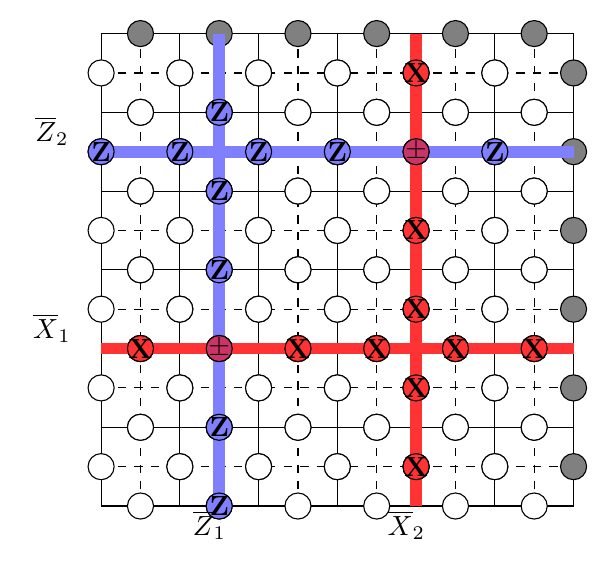
\begin{tikzpicture}
		% Draw dashed lines
		\foreach \i in {-3,-2.5,...,3}
		{
			\draw[dashed] (\i,-3) -- (\i,3);
		}
		\foreach \j in {-3,-2.5,...,3}
		{
			\draw[dashed] (-3,\j) -- (3,\j);
		}
		
		
		
		% Draw solid grid and nodes with circles in the middle of each side
		\draw[step=1cm] (-3,-3) grid (3,3);
		\foreach \i in {-2.5,...,2.5}
		{
			\foreach \j in {-2.5,...,2.5}
			{
				
				
				\begin{scope}[transform canvas={xshift=\i cm,yshift=\j cm}]
					\node[right,xshift=0.2cm,yshift=0.4cm] {};
					% Convert \j and \i to integers
					\pgfmathtruncatemacro{\intj}{\j}
					\pgfmathtruncatemacro{\inti}{\i}
					
					% Draw circles at the midpoints of each side
					\ifnum\intj=2
					\draw node[draw,circle,fill=gray] at (0,0.5) {};
					\else
					\draw node[draw,circle,fill=white] at (0,0.5) {};
					\fi
					
					\ifnum\inti=2
					\draw node[draw,circle,fill=gray] at (0.5,0) {};
					\else
					\draw node[draw,circle,fill=white] at (0.5,0) {};
					\fi
					
					\draw node[draw,circle,fill=white] at (0,-0.5) {};
					\draw node[draw,circle,fill=white] at (-0.5,0) {};
				\end{scope}
			}
		}
		
		\foreach \i in {-1.5,...,-1.5} %column
		{
			
			\draw[blue!50, line width=1.5mm] (\i,-3) -- (\i,3);
			%\node[draw, circle, fill=blue!50,label=center:\textbf{Z}] at (\i,3) {};
			\node[draw, circle, fill=blue!50,label=center:\textbf{Z}] at (\i,2) {};
			\node[draw, circle, fill=blue!50,label=center:\textbf{Z}] at (\i,1) {};
			\node[draw, circle, fill=blue!50,label=center:\textbf{Z}] at (\i,0) {};
			\node[draw, circle, fill=purple!50,label=center:\textbf{$\pm$}] at (\i,-1) {};
			\node[draw, circle, fill=blue!50,label=center:\textbf{Z}] at (\i,-2) {};
			\node[draw, circle, fill=blue!50,label=center:\textbf{Z}] at (\i,-3) {};
			
			\node[label={[anchor=south, inner sep=2pt]left:\textbf{$\overline{Z}_1$}}] at (\i,-3.5) {};
		}
		\foreach \j in {1.5,...,1.5}
		{
			
			\draw[blue!50, line width=1.5mm] (-3, \j) -- (3, \j);
			\draw node[draw,circle,fill=blue!50,label=center:\textbf{Z}] at (2,\j) {};
			\draw node[draw,circle,fill=purple!50,label=center:\textbf{$\pm$}] at (1,\j) {};
			\draw node[draw,circle,fill=blue!50,label=center:\textbf{Z}] at (0,\j) {};
			\draw node[draw,circle,fill=blue!50,label=center:\textbf{Z}] at (-1,\j) {};
			\draw node[draw,circle,fill=blue!50,label=center:\textbf{Z}] at (-2,\j) {};
			\draw node[draw,circle,fill=blue!50,label=center:\textbf{Z}] at (-3,\j) {};
			
			\node[label={[anchor=south, inner sep=2pt]left:\textbf{$\overline{Z}_2$}}] at (-3.5,\j) {};
			
		}
		
		
	
		\foreach \j in {-1,...,-1}
		{
			
			\draw[red!80, line width=1.5mm] (-3, \j) -- (3, \j);
			\draw node[draw,circle,fill=red!80,label=center:\textbf{X}] at (2.5,\j) {};
			\draw node[draw,circle,fill=red!80,label=center:\textbf{X}] at (1.5,\j) {};
			\draw node[draw,circle,fill=red!80,label=center:\textbf{X}] at (0.5,\j) {};
			\draw node[draw,circle,fill=red!80,label=center:\textbf{X}] at (-0.5,\j) {};
			\draw node[draw,circle,fill=purple!80,label=center:\textbf{$\pm$}] at (-1.5,\j) {};
			\draw node[draw,circle,fill=red!80,label=center:\textbf{X}] at (-2.5,\j) {};
			
			\node[label={[anchor=south, inner sep=2pt]left:\textbf{$\overline{X}_1$}}] at (-3.5,\j) {};
			
			
		}
		\foreach \i in {1,...,1}
		{
			
			\draw[red!80, line width=1.5mm] (\i,-3) -- (\i,3);
			\node[draw, circle, fill=red!80,label=center:\textbf{X}] at (\i,2.5) {};
			\node[draw, circle, fill=purple!80,label=center:\textbf{$\pm$}] at (\i,1.5) {};
			\node[draw, circle, fill=red!80,label=center:\textbf{X}] at (\i,0.5) {};
			\node[draw, circle, fill=red!80,label=center:\textbf{X}] at (\i,-0.5) {};
			\node[draw, circle, fill=red!80,label=center:\textbf{X}] at (\i,-1.5) {};
			\node[draw, circle, fill=red!80,label=center:\textbf{X}] at (\i,-2.5) {};
			
			\node[label={[anchor=south, inner sep=2pt]left:\textbf{$\overline{X}_2$}}] at (\i,-3.5) {};
			
			%
			
		}
		
		
	\end{tikzpicture}
\end{center}

\end{document}
